%# -*- coding: utf-8-unix -*-
% !TEX program = xelatex
% !TEX root = ../thesis.tex
% !TEX encoding = UTF-8 Unicode

\subsection{实验}
\label{sec:schema-eval}

本节中,我们首先对推理出的模式图进行直接的质量测评,
然后使用主宾语预测和三元组分类这两个任务定量评估模式图的语义表达能力,
最后我们分析一些错误例子,讨论当前模型的不足之处。

\subsubsection{实验设置}

\textbf{知识库:}
为了和已有的知识库向量表示方法进行公平比较,
我们在实验中使用了两个Freebase的子集:{\bf FB3m}以及{\bf FB15k}。
%We use three knowledge bases throughout our experiments:
%FB15k, FB15k-type and FB (full version).
%FB15k \cite{bordes2013translating} is a widely used benchmark dataset in the task of link prediction and triple classification.
FB15k由Bordes等人提出\cite{bordes2013translating},
它包含了14,951个实体,1345种不同谓词,以及483,142个事实三元组。
FB15k的三元组被分为了训练集、验证集、测试集三部分,
我们仅选用训练集部分作为使用的知识库。
%since all evaluating triples come from OpenIE system.
%Note that FB15k doesn't contain IsA relationship, thus we construct
%a new knowledge base called FB15k-type by adding type information
%of all entities into FB15k.
%Besides, we use Freebase dump of June 2015~\cite{freebase:datadumps}
%as the full version of FB.
%We use these two complementary knowledge bases in link prediction task.
%\tabref{tab:fb-size} shows the statistics of these KBs.
与此同时,我们从Freebase2015年6月的版本抽取出最主要的3,000,000个不同的实体,
并提取这些实体之间的联系,构成FB3m子集。
FB3m包含大约50,000,000个三元组,是FB15k的100倍。
和完整的Freebase相比,FB3m更加轻量化,但依然包含了大量有价值的信息。


\textbf{关系数据集}:
我们使用了三个不同的关系数据集进行知识库补全的相关实验。
在自然语言场景中,目标关系来源于开放式信息抽取系统PATTY\cite{nakashole2012patty},
包含了大约200,000种不同的自然语言关系,以及百万级别以上的三元组。
由于PATTY使用维基百科作为语料库,三元组中的所有实体均为维基百科页面,
因此每个实体均自动链接至Freebase。
我们从PATTY中抽取子集``\textbf{PATTY-100}'' 以及``\textbf{PATTY$^+$-100}'' 用于实验,
%每个数据集均包含100个自然语言关系。
PATTY-100数据集与FB15k相匹配,其包含了100个具有较多数量三元组的关系,
且三元组中所有实体均存在于FB15k中,平均每个关系包含180个关系实例。
相对应地,PATTY$^+$-100与FB3m相匹配,同样包含100个自然语言关系,平均每个关系包含388个实例。
%It is sampled from all of PATTY and may contain more complex and long-tail relations.
%From top 1,000 distinct PATTY relations sorted by the number of
%relation instances where both arguments are linked to FB15k,
%we randomly pick 100 relations for evaluation. %, called ``PATTY-100''.
%On average, each relation in PATTY-100 contains 180 instances linked to FB15k,
两个数据集中,每一个关系的三元组均被分为训练集、验证集、测试集(64\% : 16\% : 20\%)。
第三个关系数据集属于知识库场景,
我们从FB15k的``people'' 、``location'' 以及``sports'' 三个领域内挑选出37个热门谓词,
并将它们的所有三元组抽取出,组合为数据集``\textbf{FB15k-37}'' 。
每一个三元组出现在训练集、验证集、测试集的位置与FB15k保持一致。
FB15k-37是FB122\cite{guo2016jointly}的一个子集,
保证其中每一个关系在测试集中都具有至少10个三元组。
%Experiments on FB15k-37 treats our system as a classic KBC system.

%	\caption{Statistics of Freebase used in experiments. \KQ{to be updated.}}
%	\begin{tabular}{|c|c|c|c|}
%		%\toprule
%		\hline
%		Dataset				&	FB15k	&	FB15k-type	&	 FB		\\
%        \hline
%		%Ordinary entities	& 50,718,028	& 3,000,000		&		\\
%        %\hline
%        %Mediator entities	& 36,131,437	& 7,301,261		&		\\
%		%\hline
%		Total entities		&	14,951	&	14,951	&	86,849,465	 \\
%		\hline
%		Distinct relations	&	1,345	&	1,345	&	4,932	\\
%        \hline
%		Types 				&	0		&	xxxx	&	2,071	\\
%		\hline
%		IsA relationships	&	0		&	yyyy	&	zzzz	\\
%		\hline
%		Triple facts		&	483,142	&	483,142	& 280,788,583	\\
%		\hline
%	\end{tabular}%
%	\label{tab:fb-size}%
%\end{table}

\textbf{用于比较的已有方法:}
对于知识库向量表示的方法,我们与TransE\cite{bordes2013translating},
KALE\cite{guo2016jointly},TEKE \cite{wang2016text}以及
HOLE\cite{nickel2015holographic}进行比较。
%TransE models the confidence of a triple fact as vector translations on the
%embeddings of the predicate and two entity arguments.
%%TransE models a relationship as operating translations on the embeddings of
%%subject and object entities. \KQ{Change all subject, object into head, tail??}
%KALE and TEKE are two extensions of TransE.
%KALE introduces logical rules as the combination of atom triple facts with logical connectives,
%therefore the model can learn embeddings from both positive triples and rules.
%TEKE enables each relation to own different representations for different subject and object
%entities, by leveraging the rich context information of a triple fact from web text corpus.
%HOLE is a novel compositional embedding model for representing relationships,
%which is based on the circular correlation of entity vectors.
%
对于规则推导的方法,我们与
SFE\cite{gardner2015efficient}以及AMIE+\cite{galarraga2015fast}这两个系统进行比较。
%One traditional model, called Path Ranking Algorithm \cite{lao2011random},
%extracts all possible paths connecting subject and object entities,
%then learns a feature-based model to represent each relation,
%and SFE is an extension of PRA model, by adding extra subgraph features
%from the surrounding of subject and object entities in the knowledge base.
%AMIE+ first searches possible structures, and then calculates the confidence score
%of each structure by a simple counting strategy in positive triple facts
%(without the step of weight learning).
我们考虑使用CPRA模型\cite{wang2016knowledge}作为另一个比较方法。
但在PATTY相关的数据集中,不同关系之间几乎不存在相同的实体对,
因此CPRA模型将会退化为传统的PRA模型\cite{lao2011random},
被更优秀的SFE严格取代。
这些模型在\secref{sec:rw-kbc}或\secref{sec:schema-related}中已有论述。

\textbf{模型实现细节:}
我们评估了模型的两个变种,分别为生成带限制的模式图的Ours-SC,
以及仅生成简单模式图的Ours-SK。
%The only difference between them is whether
%to explore constraints in schema generation (\secref{sec:candgen}).
%Ours-SK only picks skeletons as candidates (without searching for constraints),
%while Ours-SC is allowed to use all candidate schemas.
%We evaluate our approach under several settings.
%In candidate generation step, we compare two settings:
%``use-skeleton-only'' and ``use-whole-schema'', based on
%whether to explore constraints.
%The first specification only extract path candidates without generating
%constraints, while the latter one is free to use all candidate schemas.
%In schema inference step, we compare two strategies ``random walk''
%and ``zero-one'', described in \secref{sec:schema}.
以下是具体调参细节:
\begin{itemize}
\item{候选模式图的数量,即优先队列容量$B$设为5000;}
\item{模式图骨架长度限制$\tau$设为3,我们的方法可以支持更长的骨架,
但具体测试中无明显的效果提升,同时候选生成时间显著增长,这里不展开讨论;}
\item{支持率阈值$\gamma$调参范围为\{5\%, 10\%, 15\%, 20\%\};}
\item{平滑参数$\alpha$调参范围为\{1e-6, 1e-5, 1e-4\};}
\item{学习率$\eta$调参范围为\{0.02, 0.05, 0.1\}。}
\end{itemize}
用于比较的系统中,具有开源代码的方法包括AMIE+
\footnote{https://www.mpi-inf.mpg.de/departments/databases-and-information-systems/research/yago-naga/amie/},
SFE\footnote{https://github.com/matt-gardner/pra}
以及HOLE\footnote{https://github.com/mnick/scikit-kge}。
KALE的代码由作者提供,
TransE基于HOLE的代码运行,
并且我们在TransE的基础上自行实现了TEKE模型。
以上基于知识库向量表示的模型均使用最大间隔损失进行训练,
对于KALE模型,学习率调参范围为\{0.02, 0.05, 0.1\},
最大间隔参数范围为\{0.1, 0.12, 0.15, 0.2\};
对于TransE,TEKE以及HOLE,学习率调参范围为\{0.05, 0.1, 0.2\},
最大间隔参数范围为\{0.5, 1.0, 1.5, 2.0, 2.5\}。


\subsubsection{模式图质量测评}
这一部分的实验中,我们主要关注具有明确结构的模式图是否
可以弥补Freebase和PATTY$^+$-100之间的语义差距。
我们首先通过具体的例子观察不同的规则推导方法,
即Ours-SC,Ours-SK,AMIE+以及SFE所生成的代表性结构。
我们从PATTY$^+$-100数据集中挑选出四个具有一定复杂性的关系,
并在较大结构的FB3m上学习各自的规则。
对于Ours-SC和Ours-SK,我们使用选择概率最高的模式图作为代表性结构。
SFE模型中,每个规则(谓词路径)都对应一个特征,
我们选择特征权重最高的规则作为代表性结构。
AMIE+依靠准确率对规则进行排序,因此我们挑选准确率最高的规则,
若多个规则准确率相同,我们则从中手动选择最合适的规则。

%TODO:可能图要重新调整,这个样子太丑陋了
\begin{figure*}[ht]
    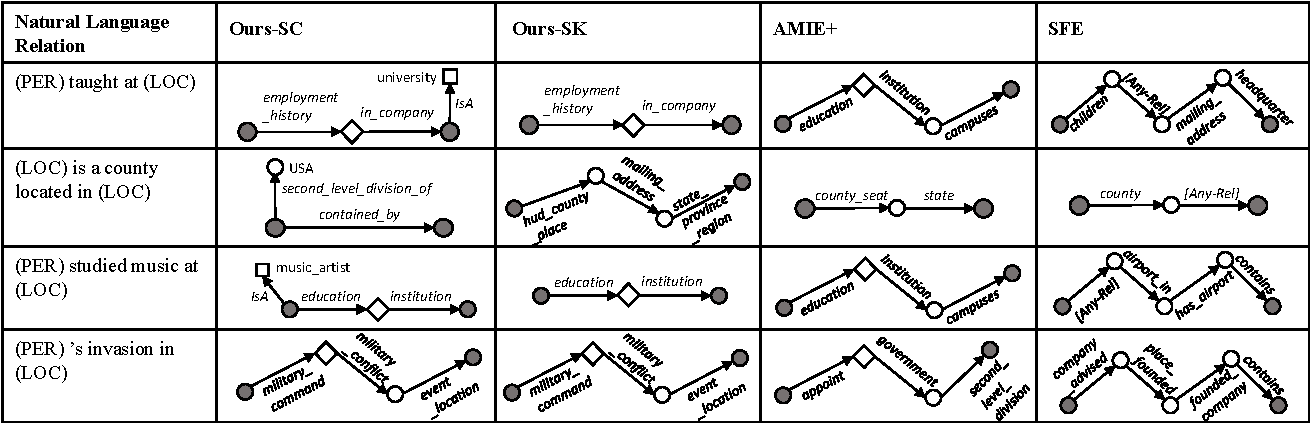
\includegraphics[width=1.0\columnwidth]{figure/schema/case-crop.eps}
    \centering
    \bicaption{不同的规则推导系统对四个复杂关系生成的代表性结构。}
    {Top structures produced by four systems on 4 complex relations.}
    \label{fig:schema-relation-example}
\end{figure*}

\figref{fig:schema-relation-example}列出了四个自然语言关系,
以及不同系统生成的最佳结构。
其中,圆点表示实体或变量,左右两个黑色圆点分别代表$x_{subj}$和$x_{obj}$。
方块代表知识库中的类型,菱形则代表用于维护多元关系的辅助节点。
%TODO: 如果篇幅不够,拿IJCAI的note来凑
从这些例子中可以发现,Ours-SC的模式图所具有的分支结构,可以带来更加精确的语义。
对比仅生成骨架的Ours-SK,带有限制的查询图在每个例子上都表达了几乎完全正确的语义。
另一方面,AMIE+和SFE输出的最佳结构不尽如人意。
AMIE+按照准确率对规则排序,因此总是倾向于更具体的规则,但牺牲了召回率。
同时随着规则长度提升至4甚至更高,AMIE+系统消耗了大量内存,无法返回任何结果。
SFE生成的规则中包含\textit{[Any-Rel]}代表任意谓词,因此可以生成更多灵活的路径作为特征,
但显然其中的大部分都不具有清晰的语义,人类难以直接理解。

作为补充实验,我们对Ours-SC和Ours-SK生成的模式图进行了人工测评。
对每一个自然语言关系,我们从中抽取出至多前5个概率值至少为0.05的模式图,
并由三位%熟悉Freebase结构的
标注者进行人工打分,
分值选择范围为\{0, 0.5, 1\},
分别代表 ``{不相关模式图}'' (骨架层次已出现语义偏离),
``{部分匹配}'' (骨架语义正确,但其余限制需要改善)以及
``{完全匹配}'' (骨架和限制的语义均无明显偏差)。
我们将三位标注者的打分进行平均,得到每一个模式图的标注分值,
并计算排名前$n$的所有模式图的平均分值,记做AvgSc@$n$。
三位标注者之间的Kappa系数为0.541,具有稳定的相关性。
\tabref{tab:average-score}列出了不同的AvgSc@$n$分值,
Ours-SC在骨架的基础上挖掘额外的语义限制,将结果提高了约13\%。

\begin{table}[ht]
	\centering
	\bicaption{模式图列表的AvgSc@$n$测评结果。}{AvgSc@$n$ results on top-ranked schemas.}
	\label{tab:average-score}
	\begin{tabular}{c|ccc}
		\hline
						&	n=1		&	n=3		&	n=5			\\
		\hline
		Ours-SK			&	0.44	&	0.37	&	0.34		\\
		Ours-SC			&	\textbf{0.47}	&	\textbf{0.40}	&	\textbf{0.38} \\
		\hline
	\end{tabular}
\end{table}


\subsubsection{主宾语预测任务测评}
主宾语预测任务的目标是预测三元组($e_{subj}$, $r$, $?$)或($?$, $r$, $e_{obj}$)
所缺失的宾语或主语。
测试集中的每一个三元组都对应两个这样的预测任务。
\eqnref{eqn:score-def}代表着给定一端实体,生成另一端未知实体的概率,
因此对每一个带有未知实体的待预测三元组,我们根据该公式计算生成不同实体的概率,
并衡量答案实体的概率排名高低。
我们在实验中使用了两个评价指标,分别为MRR和Hits@$n$,
前者衡量答案实体在所有预测任务中的平均排名,
后者关注在多少比例的预测任务中,答案实体的概率排在前$n$位。
不同的实验方法通过验证集的MRR分值进行独立调参。

以上对排名高低的衡量暗含着一个假设:除了答案实体之外,其余实体均为错误实体。
然而考虑到关系可能具有的一对多性质,对于一个待预测的三元组,
除了答案实体之外,还可能存在其它实体与给定的已知实体匹配,
严格来讲,这些实体虽然不同于唯一的答案,但也不应该算作错误。
因此,我们使用和TransE\cite{bordes2013translating}相同的设定,
在测评中引入两种不同的模式,分别为原始模式和过滤模式:
在过滤模式中,计算每个预测的答案实体排名时,均忽略不同于答案的其余正确实体,
因此过滤模式下,排名值可能会提高;而原始模式则不做任何的过滤。

%
%We perform the evaluation on FB15k under filtered setting \KZ{What is this
%setting? Never mentioned before?}.
%\figref{fig:trend-with-budget} shows how the MRR results
%\KQ{on validation set}, vary with the number of candidate schemas.
%From the results, we observe that:
%1) The MRR result increases with the number of candidate schemas in
%every setting, which indicates that larger number of candidates
%leads to a better model.
%2) Compare with strategies on candidate generation, use-whole-schema
%outperforms use-skeleton-only, demonstrating the capability of constraints
%to represent natural language relations.
%3) \KQ{random walk v.s. zero-one, need to get real results before the analysis.}
%
%%\KQ{Figure to be plotted: budget 1k~5k  *  4 different specifications.}
%\begin{figure}[th]
%\epsfig{file=trend.eps, width=0.65\columnwidth}
%\centering
%\caption{
%	The trend of link prediction results on FB15k (filtered setting).
%	X axis: size of priority queue,
%	Y axis: MRR score. \KQ{content to be updated.}
%}
%\label{fig:trend-with-budget}
%\end{figure}

%We first evaluate our approach and state-of-the-art systems on PATTY-100 relations.
%Then we compare our approach with state-of-the-art models.
%\KQ{Need to say a little bit about the parameters we used here.}
%\tabref{tab:link-pred-patty} %and \tabref{tab:link-pred-filtered}
%shows the link prediction results on FB15k.

%\KZ{Due to memory issues of the code, SFE method failed to produce any result.
%This is a bit strange: you pick SFE as a comparison but it doesn't work for
%link prediction at all! Better fix this!}
%As we can see, our approach outperforms both embedding and
%other rule induction models.

我们使用FB15k作为知识库进行实验,并与其余模型进行比较。
在接下来的实验中,为了方便比较,
我们的模型同一参数$\gamma=10\%$,$\alpha=1e-4$,以及$\eta=0.1$,
对应着PATTY-100验证集上,在过滤模式下的最高MRR结果。
\tabref{tab:link-pred-patty}和\tabref{tab:link-pred-fb15k}
分别展示了在PATTY-100和FB15k-37数据集上的实验结果。
在两个数据集上,SFE模型的代码均碰到了内存问题,
因此表格中没有列出对应的结果。
对于PATTY-100中的关系,我们基于模式图的语义表示方法,
其效果优于其它用于比较的规则推导与知识库向量表示模型,
以及仅生成简单模式图的变种。
在FB15k-37数据集上,Ours-SC与Ours-SK的结果十分接近,
这主要是因为知识库上的一部分谓词具有等价形式,
例如$location.location.containedby$和$location.location.contains$
互为相反关系,对于这些关系,只需要依靠骨架结构就可以精确描述语义。
对比两张表格可以发现,对于所有不同的模型和实验模式,
自然语言关系上的主宾语预测结果都低于对应的知识库谓词上的结果。
%Comparing the results on different set of relations,
%the improvements on complex relations are much more significant than those
%on ordinary relations, indicating the usefulness of the extra constraints
%in representing complex relations.
%Besides, the link prediction results on natural language relations
%are relatively lower than
%those results evaluated on FB15k relations \cite{guo2016jointly}.
主要原因有两点:
1) FB15k-37上的每一个谓词平均包含接近千级别的训练三元组,
而PATTY-100中的每个关系平均只有115个训练数据;
2) 自然语言关系具有更多歧义,开放式信息抽取的结果会包含多种语义,
而且还要考虑抽取错误的情况,
相比之下,知识库上的谓词及三元组的制定经过了部分人工干预,因此歧义更少。


\begin{table}[b]
	\centering
	\bicaption{在PATTY-100上进行主宾语预测的测评结果。}{Link prediction results on PATTY-100 relations.}
	\label{tab:link-pred-patty}
	\begin{tabular}{c|ccc|ccc}
		\hline
				&	\multicolumn{3}{c|}{Raw}
				&	\multicolumn{3}{c}{Filtered}	\\
		\cline{2-7}	
				&	MRR	&	H@3	&	H@10
				&	MRR	&	H@3	&	H@10		\\
		\hline
		TransE
				&	0.112	&	12.4	&	27.1
				&	0.129	&	14.5	&	29.9	\\	%m1.75_lr0.10
		KALE
				&	0.112	&	12.5	&	25.4
				&	0.125	&	14.4	&	27.5	\\	%Test-base-k100-d0.15-ge0.02-gr10-filt.eval_KQ
		TEKE
				&	0.101	&	10.9	&	24.1
				&	0.114	&	12.6	&	26.3	\\
		HOLE
				&	0.109	&	10.5	&	23.3
				&	0.121	& 	12.3	&	25.8	\\	%log.hole_d100_m0.25_lr0.05
		%AMIE+
		%		&	0.119	&	23.5
		%		&	0.132	&	24.4	\\
		AMIE+
				&	0.148	&	16.5	&	29.3
				&	0.174	&	19.5	&	\textbf{31.9}	\\
		\hline
		Ours-SK
				&	0.169	&	18.2	&	29.3
				&	0.179	&	19.1	&	30.4	\\		%Blackhole
		Ours-SC
				&	\textbf{0.172}		&	\textbf{18.5}	&	\textbf{29.8}
				&	\textbf{0.185}		&	\textbf{19.9}	&	31.5	\\	%Blackhole
		\hline
	\end{tabular}
\end{table}

%\begin{table*}[ht]
%	\small
%	\centering
%	\caption{Link prediction results on FB15k (raw setting).}
%	\begin{tabular}{|c|ccccc|ccccc|ccccc|}
%		%\toprule
%		\hline
%				&	\multicolumn{5}{c|}{Complex relations}
%				&	\multicolumn{5}{c|}{Ordinary relations}
%				&	\multicolumn{5}{c|}{Overall}	\\
%		\cline{2-16}	
%		\multirow{2}{*}{}	&	\multirow{2}{*}{MRR}	&	\multirow{2}{*}{MED}	&	\multicolumn{3}{c|}{Hit@n(\%)}
%							&	\multirow{2}{*}{MRR}	&	\multirow{2}{*}{MED}	&	\multicolumn{3}{c|}{Hit@n(\%)}
%							&	\multirow{2}{*}{MRR}	&	\multirow{2}{*}{MED}	&	\multicolumn{3}{c|}{Hit@n(\%)}	\\
%				&	&	&	3	&	5	&	10	
%				&	&	&	3	&	5	&	10	
%				&	&	&	3	&	5	&	10	\\
%		\hline
%		TransE
%				&	0.089	&	75.0	&	11.7	&	17.2	&	23.2
%				&	0.081	&	66.0	&	 8.1	&	12.1	&	19.6
%				&	0.082	&	68.0	&	 8.9	&	13.2	&	20.4	\\
%		KALE	
%				&	0.142	&	47.0	&	17.5	&	23.4	&	30.5
%				&	0.104	&	42.0	&	11.2	&	16.0	&	24.0
%				&	0.112	&	\textbf{43.0}	&	12.5	&	17.6	&	25.4	\\
%		TEKE	
%				&	0.119	&	68.4	&	14.7	&	19.5	&	27.6
%				&	0.096	&	57.2	&	9.8  	&	14.6	&	23.1
%				&	0.101	&	59.0	&	10.9	&	15.7	&	24.1	\\
%		HOLE
%				&	0.153	&	55.0	&	16.0	&	20.5	&	27.4
%				&	0.097	&	51.0	&	 9.1	&	13.9	&	22.2
%				&	0.109	&	52.0	&	10.5	&	15.4	&	23.3	\\
%		%\hline
%		%SFE-AnyRel
%		%SFE-OneSide
%		AMIE+
%				&	0.164	&	76.3	&	18.2	&	21.9	&	26.6
%				&	0.107	&	68.3	&	11.3	&	15.8	&	22.6
%				&	0.119	&	69.5	&	12.7	&	17.1	&	23.5	\\
%		Ours
%				&	0.225	&	42.5	&	24.3	&	27.8	&	34.7
%				&	0.158	&	43.0	&	16.9	&	21.0	&	28.5
%				&	\textbf{0.172}	&	\textbf{43.0}	&	\textbf{18.5}	&	\textbf{22.5}	&	\textbf{29.8}	\\
%		\hline
%	\end{tabular}
%	\label{tab:link-pred-raw}
%\end{table*}

\begin{table}[tbh]
	\centering
	\bicaption{在FB15k-37上进行主宾语预测任务的测评结果。}{Link prediction results on FB15k-37 relations.}
	\label{tab:link-pred-fb15k}
	\begin{tabular}{c|ccc|ccc}
		\hline
				&	\multicolumn{3}{c|}{Raw}
				&	\multicolumn{3}{c}{Filtered}	\\
		\cline{2-7}	
				&	MRR	&	H@3	&	H@10
				&	MRR	&	H@3	&	H@10	\\
		\hline
		TransE
				&	0.310			&	39.3	&	53.2
				&	0.394	&	52.5	&	65.0	\\	%log.transe_m2.00_lr0.10.train_lp
		KALE
				&	0.342	&	40.6	&	53.0
				&	0.410	&	48.7	&	60.6	\\	%Test-KALE-1110-k100-d0.12-rd0.12-ge0.05-gr10-w1(0.1)-w2(1)-w3(0)-w4(0)-filt.eval_KQ
		TEKE
				&	0.288	&	35.7	&	49.2
				&	0.339	&	43.0	&	56.5	\\
		HOLE
				&	0.234	&	26.7	&	39.5
				&	0.323	& 	36.5	&	50.5	\\	%log.hole_m0.25_lr0.10.train_lp
		AMIE+
				&	0.395	&	46.1	&	53.7
				&	0.562	&	60.0	&	68.9	\\
		\hline
		Ours-SK
				&	0.425	&	47.8	&	55.6
				&	0.664	&	68.8	&	73.0	\\		%Darkstar
		Ours-SC
				&	\textbf{0.427}		&	\textbf{48.1}	&	\textbf{55.7}
				&	\textbf{0.671}		&	\textbf{69.3}	&	\textbf{73.3}	\\		%Darkstar
		\hline
	\end{tabular}
\end{table}

%\begin{table*}[ht]
%	\small
%	\centering
%	\caption{Link prediction results on FB15k (filtered setting).}
%	\begin{tabular}{|c|ccccc|ccccc|ccccc|}
%		%\toprule
%		\hline
%				&	\multicolumn{5}{c|}{Complex relations}
%				&	\multicolumn{5}{c|}{Ordinary relations}
%				&	\multicolumn{5}{c|}{Overall}	\\
%		\cline{2-16}	
%		\multirow{2}{*}{}	&	\multirow{2}{*}{MRR}	&	\multirow{2}{*}{MED}	&	\multicolumn{3}{c|}{Hit@n(\%)}
%							&	\multirow{2}{*}{MRR}	&	\multirow{2}{*}{MED}	&	\multicolumn{3}{c|}{Hit@n(\%)}
%							&	\multirow{2}{*}{MRR}	&	\multirow{2}{*}{MED}	&	\multicolumn{3}{c|}{Hit@n(\%)}	\\
%				&	&	&	3	&	5	&	10	
%				&	&	&	3	&	5	&	10	
%				&	&	&	3	&	5	&	10	\\
%		\hline
%		TransE
%				&	0.097	&	69.0	&	13.0	&	18.7	&	25.0
%				&	0.092	&	62.0	&	 9.7	&	14.2	&	22.2
%				&	0.094	&	63.0	&	10.4	&	15.2	&	22.8	\\
%		KALE	
%				&	0.153	&	43.0	&	19.9	&	25.5	&	32.5
%				&	0.118	&	39.0	&	12.9	&	18.0	&	26.1
%				&	0.125	&	\textbf{39.0}	&	14.4	&	19.6	&	27.5	\\
%		TEKE	
%				&	0.129	&	64.3	&	16.2	&	21.4	&	29.1
%				&	0.109	&	52.7	&	11.7	&	16.9	&	25.6
%				&	0.114	&	54.0	&	12.6	&	17.9	&	26.3	\\
%		HOLE
%				&	0.162	&	50.5	&	17.4	&	21.8	&	29.0
%				&	0.109	&	47.0	&	10.9	&	16.1	&	24.9
%				&	0.121	&	47.0	&	12.3	&	17.3	&	25.8	\\
%		%\hline
%		%SFE-AnyRel
%		%SFE-OneSide
%		AMIE+
%				&	0.180	&	73.8	&	18.6	&	22.4	&	27.5
%				&	0.120	&	63.5	&	12.5	&	17.0	&	23.6
%				&	0.132	&	65.0	&	13.8	&	18.2	&	24.4	\\
%		Ours
%				&	0.237	&	41.0	&	25.2	&	29.1	&	35.5
%				&	0.171	&	40.0	&	18.4	&	22.4	&	30.5
%				&	\textbf{0.185}	&	40.0	&	\textbf{19.9}	&	\textbf{23.8}	&	\textbf{31.5}	\\
%		\hline
%	\end{tabular}
%	\label{tab:link-pred-filtered}
%\end{table*}





\subsubsection{三元组分类任务测评}
三元组分类任务的目标是预测一个未知三元组($e_1$, $r$, $e_2$)是否描述了一个正确的客观事实。
考虑到这是个二分类任务,测试数据中需要包含负样本三元组,
因此我们使用和KALE\cite{guo2016jointly}相同的生成策略,
对测试集和验证集中的每个三元组生成10个不同的负样本,
其中5个三元组替换了主语,另外5个替换了宾语。
为了保证负样本不至于显得过于错误,
我们保证用于替换的主语(或宾语)都曾出现在目标关系的某个已知三元组的同样位置上。

对于每一个目标关系,我们通过\eqnref{eqn:likelihood-def}计算各个未知三元组的似然值,
以此作为置信度对所有测试集的所有正负样本进行排序。
我们使用FB15k作为知识库进行了实验,
并使用MAP(Mean Average Precision)作为测评指标,
衡量不同的模型在三元组分类任务上的效果。
%TODO: 找个地方说一下评价指标
\tabref{tab:triple-clsf}列出了PATTY-100和FB15k-37数据集上的效果,
我们的模型在两个数据集上均大幅度优于其它方法。
此外我们发现,仅生成简单模式图的方法效果要优于生成完整模式图的做法。
我们对实验数据进行了分析,
造成这个现象的原因源于负样本生成方式的天然缺陷。
例如对于 ``father of'' 关系,我们期望负样本中能包含表示母子关系的实例,
识别这种负样本需要较高难度,必须依靠额外限制才能和正样本进行区分。
然而,负样本的生成方式决定了主语只能替换为某个随机小孩的父亲,
判断三元组正确与否主要依靠骨架的正确性,
因而很难体现模式图的额外限制为给语义理解带来的优势,
减少候选模式图的数量和复杂度反而能得到更好的效果。


%(what we generated in the current experimental setting)
%as negative data makes the classification problem harder, and shows the value of constraints.
%While in link prediction, the constraints play an important role to 
%rank positive entities higher.
%Moreover, we find that there's almost no difference
%between our two variances on FB15k-37, that's not unexpected because skeletons
%are enough to represent the majority of these predicates.


%Observing results of each model, it's interesting to find that all rule induction models
%performs much better than embedding techniques, which reveals us that
%explicit semantic feature mining could help to find more precise representations,
%especially when the training data is small.
%Ours-SC outperforms the other embedding methods on PATTY-100 dataset, demonstrating the
%importance of constraints. However, the gap could be bigger if the negative triples
%are generated to distinguish the constraints, e.g., for father-of relation,
%using a child's own mother instead of a random father or a random mother as negative data.

\begin{table}[tbh]
	\centering
	\bicaption{三元组分类任务的MAP测评结果。}{MAP results on triple classification task.}
	\begin{tabular}{c|cc}
		%\toprule
		\hline
							& PATTY-100	&	FB15k-37 	\\
        \hline
		TransE				&	0.304	&	0.666	\\	% m0.25, lr0.05	|	m1.00, lr0.10
		KALE				&	0.309	&	0.654	\\
		TEKE				&	0.282	&	0.631	\\
		HOLE				&	0.308	&	0.680	\\	% m0.25, lr0.20	|	m0.20, lr0.10
		SFE					&	0.329	&	0.621	\\	% due to data shrinking ...
		AMIE+				&	0.226	&	0.730	\\	
		\hline
		Ours-SK				&	\textbf{0.408}	&	\textbf{0.804}	\\	
		Ours-SC				&	0.403	&	0.803	\\
		\hline
	\end{tabular}
	\label{tab:triple-clsf}
\end{table}



\subsubsection{错误分析}

%\figref{fig:relation-example} shows the paraphrasing results of
%selected relations.
%Show a case-by-case P/R/F1/RR?
%The results of top-ranked schemas show us that our paraphrasing system
%is able to produce concrete and precise structural representations.
对于一些自然语言关系,我们的模型可能难以寻找出较为正确的模式图。
我们对结果进行了分析,并总结出以下几类主要错误。

1. 开放式信息抽取提供的关系三元组存在错误。
考虑到PATTY主要利用依存语法分析对句子进行关系识别,
语法分析本身的偏差将导致生成错误的三元组。
例如对于关系\textit{``served as''},给定句子
\textit{``Dennison served as the 24th Governor of Ohio and as U.S. Postmaster General ...''},
PATTY提取的实体对(William Dennison Jr., Ohio)
有误,正确的宾语应为``Governor of Ohio'' 。

2. PATTY数据集中,每个关系实际代表着一个关系同义集,即由多个具有相似结构的关系组成的组合,
这导致部分关系同义集混入了语法相似但语义不同的关系,产生本不存在的歧义。
以PATTY中的关系同义集\textit{``'s wife''}为例,
其中混入了少部分可能由\textit{``the wife of''}产生的三元组,其中主语为妻子,宾语反而为丈夫。
%由于PATTY并未提供原句,因此不能直接对关系同义集里的内容进行过滤。
在混入的三元组干扰下,模型会误以为该关系的准确语义为不带有性别限制的配偶关系,
因此正确的模式图很难获得较高的概率。
%These instances are due to another pattern in the synset,
%\textit{``the wife of''}, which gives the exact opposite semantics.
%though our system is able to filter out noisy instances, the learned schema
%distribution would be affected if the percentage of noisy data is large.

3. 对于部分关系,知识库本身缺乏用于描述其语义的谓词。
对于一些琐碎的自然语言关系例如\textit{``talk to''},知识库显然不包含这类事实。
但即便对于一些不那么琐碎的关系,知识库依然可能缺乏必要的谓词。
例如关系\textit{``(singer) performed in (LOC)''}	% synset 0246
描述的是歌手和演唱会举办地的联系,但Freebase中并不包含类似于
\textit{place\_visited}或\textit{hold\_concerts\_in}的谓词,
因此难以通过已有知识表示目标关系的语义。

4. 由于搜索空间的限制,部分有意义的模式图无法在候选生成步骤被过滤。
例如关系\textit{``(actor) starring with (actor)''},
由于Freebase通过辅助节点(Mediator)维护多元关系,
这使得最合适的骨架\footnote{
骨架具有$actor \rightarrow med. \rightarrow film \rightarrow med. \rightarrow actor$
形式,其中$med.$为辅助节点。}长度为4,并不满足候选生成的骨架长度限制,因此模型无法得到这样的模式图。

%\KZ{This is why I said we should evaluate the impact of $\tau$.}
%
%\KZ{After reading this paper, one thing that puzzles me is that why is this
%method called paraphrasing natural language relations to knowledge base? The
%approach you are proposing can be used for ordinary KB completion task, right?
%In other words we are not making use of the natural language feature at all.
%I think perhaps we can include some experiments you did with NL features to
%show that NL features are not necessary and explain why. This will clear the
%doubt of some readers.}

